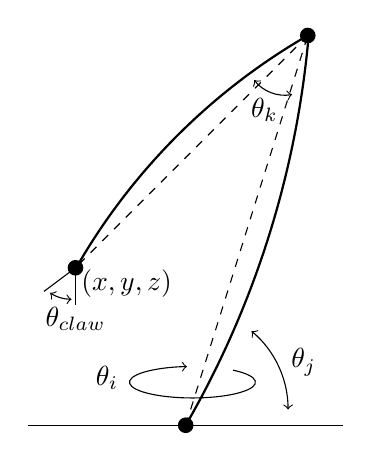
\begin{tikzpicture}
	\node[circle,fill,inner sep=-2pt] at (0,0){}; % origin/first joint
	\node[circle,fill,inner sep=-2pt] at (1.55,4.95){}; % second joint
	\node[circle,fill,inner sep=-2pt] at (-1.4,2){}; % end effector

	\draw (-2,0) -- (2,0); %base
	\draw[dashed] (0,0) -- (1.55,4.95);
	\draw[dashed] (1.55,4.95) -- (-1.4,2);


	\draw[thick,rotate=-30] (0,0) arc (0:25:12cm); % limb #1 arc
	\draw[thick] (1.55,4.95) arc (120:150:8cm); % limb #2 arc
	\draw (-1.4,2) -- (-1.8,1.7);
	\draw (-1.4,2) -- (-1.4,1.53);

	\draw[->,xscale=4] (0.15,0.7) arc (50:-265:0.2cm); % i axis rotation arc
	\draw[<->] (1.3,0.2) arc (0:50:1.3cm); % j axis rotation arc
	\draw[<->] (1.35,4.2) arc (280:218:0.5cm); % k axis rotation arc
	\draw[<->] (-1.45,1.6) arc (270:237:0.5cm); % claw rotation arc

	\node at (-1,0.6) {$\theta_{i}$}; % i axis rotation label
	\node at (1.5,0.8) {$\theta_{j}$}; % j axis rotation label
	\node at (1,4.0) {$\theta_{k}$}; % k axis rotation label
	\node at (-1.4,1.35) {$\theta_{claw}$}; % k axis rotation label
	\node at (-0.75,1.8) {${(x,y,z)}$}; % end effector labeling
\end{tikzpicture}
